\section{Curvature tensor}

Let $M$ be a Riemannian manifold. $\forall p \in M$, $\forall u,v \in T_pM$
choose a $C^{\infty}$ map
\[
c: (-\epsilon, \epsilon) \times (-\delta, \delta) \to M
\]
s.t. $u = (c^0)'(0,0)$, $v = (c^1)'(0,0)$, $p = c(0,0)$, where $c_s(t) = c^t(s) = c(s,t)$.
Define paralllel transport around the square:
\[
P_{s,t}w := P_{c^0(0)}P_{c_s(0)}P_{c^t(s)}P_{c_o(t)}w,\quad w\in T_pM.
\]
\begin{figure}[h]
    \centering
    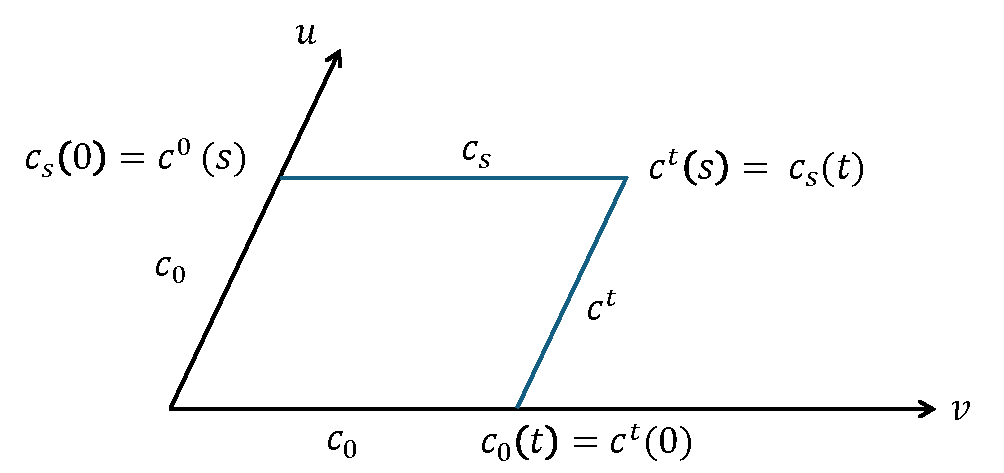
\includegraphics[width=0.5\textwidth]{graphics/parallelogram.pdf}
    \caption{Parallel transport around a parallelogram.}
\end{figure}
In Euclidean space, $P_{s,t} w = \operatorname{Id} w \forall s,t$. In general $P_{s,t}w - w \neq 0$.

\begin{lemma}
For $p \in M$ and $w \in T_pM$, the map
\[
\begin{aligned}
(-\epsilon, \epsilon) \times (-\delta, \delta) &\to T_pM \\
(s,t) &\mapsto P_{s,t}w
\end{aligned}
\]
is $C^{\infty}$ and satisifies
\[
\frac{\partial^2}{\partial s \partial t} P_{s,t}w\Bigg|_{(s,t)=(0,0)} = \lim_{(s,t)\to(0,0)}\frac{P_{s,t}w - w}{st},
\]
where the left-hand side is the Fréchet derivative for vector-valued functions.
Specifically, for an othonormal basis $e_1, \dots, e_n$ of $T_pM$,
\[
\frac{\partial^2}{\partial s \partial t} P_{s,t}w= \sum_{i=1}^n\left(\frac{\partial^2}{\partial s \partial t} \langle P_{s,t}w, e_i\rangle\right)e_i.
\]
\end{lemma}

\begin{proof}
Consider $s,t$ sufficiently small. Assume $\Im(c)$ is contained in a coordinate neighborhood $(U,\phi)$.
First, consider $P_{c_o(t)w}$. Let, 
\[
\phi(c_0(t)) = (c_0^1(t), \dots, c_0^n(t)),\quad P_{c_0(t)}w = \sum_{i=1}^n\xi^i(t)(\partial_i)_{c_0(t)},
\]
then $\xi^1(t), \dots, \xi^n(t)$ solve the linear ODE
\[
\frac{d\xi^k}{dt} + \sum_{i,j = 1}^{n}\Gamma_{ij}^k\frac{dc_0^i}{dt}\xi^j=0,\quad k=1,\dots,n,
\]
with initial condition $\sum_{i=1}^n \xi^i(0)(\partial_i)_p=w.$
Next, consider $P_{c^t(s)}P_{c_o(t)}w$. Let
\[
\sum_{i=1}^n \eta^i_t(s)(\partial_i)_{c^t(s)} = P_{c^t(s)}P_{c_0(t)}w.
\]
Then $\eta^1_t(s), \dots, \eta^n_t(s)$ solve the linear ODE
\[
\frac{d\eta^k_t}{ds} + \sum_{i,j = 1}^{n}\Gamma_{ij}^k\frac{d(c^t)^i}{ds}\eta^j_t=0,\quad k=1,\dots,n,
\]
with initial conditions $\eta_t^k(0) = \xi^k(t)$ ($k=1,\dots,n$).
By standard ODE theory, $\eta_t^k(s)$ are $C^{\infty}$ functions in $(s,t)$.
Repeating the same argument shows $P_{s,t}w$ is $C^{\infty}$ in $(s,t)$.

Fix an orthonormal basis $e_1, \dots, e_n$ of $T_pM$ and Taylor expand $\langle P_{s,t}w, e_i\rangle$ at $(s,t)=(0,0)$. Since 
$P_{s,0} = P_{0,t}w = w$,
\[
\frac{\partial^k}{\partial s^k}\langle P_{s,0},w,e_i\rangle = \frac{\partial^k}{\partial t^k}\langle P_{0,t}w,e_i\rangle = 0, \quad k\geq1.
\]
Then, $\forall i$,
\[
\langle P_{s,t}w,e_i\rangle = \langle w,e_i\rangle + st\frac{\partial^2}{\partial s\partial t}\langle P_{s,t}w, e_i\rangle\Bigg|_{(0,0)} 0 \mathcal{O}(st^2 + s^2t).
\]
It follows that
\[
\left\langle \lim_{(s,t)\to(0,0)}\frac{P_{s,t}w -w }{st},e_i\right\rangle = \frac{\partial^2}{\partial s\partial t}\langle P_{s,t}w,e_i\rangle\Bigg|_{(s,t)=(0,0)}.
\]
Multiplying by $e_i$ and summing over $i$ gives the desired result.
\end{proof}

\begin{definition}[Curvature tensor]
$\forall p \in M$, $u,v \in T_pM$, define $R(u,v) : T_pM \to T_pM$ by
\[
R(u,v)w := \frac{\partial^2}{\partial s \partial t} P_{s,t}w\Bigg|_{(s,t)=(0,0)} = \lim_{(s,t)\to(0,0)}\frac{P_{s,t}w - w}{st}, \quad w \in T_pM.
\]
The map $R:T_pM \times T_pM \times T_pM \to T_pM$ is called the \emph{curvature tensor}.
$R$ is a tensor field of type $(1,3)$.
\end{definition}

\begin{lemma}\label{lemma:8.3}
$\forall p \in M$ and $\forall w \in T_pM$, let $Z_{(s,t)} := P_{c^t(s)}P_{c_o(t)}w$. Then
\[
R(u,v)w = (\nabla_c + \nabla_{c_s}Z)\Big|_{(s,t)=(0,0)}.
\]
\end{lemma}

\begin{proof}
By \autoref{prop:covariant_derivative_along_curves_limit}, the covariant derivative along $c_s$ is 
\[
(\nabla_{c_s}Z)\Big|_{t=0} = \lim_{h\to0}\frac{P_{c_s(0)}Z(s,h) - Z(s,0)}{h}.
\]
Note that $c_0(h) = c^h(0)$ and $P_{c^h(0)}: T_{c^h(0)}M \to T_{c^h(0)}M$ is the identity map.
Since $P_{c_0(h)}: T_pM \to T_{c_0(h)}$ and $P_{c_0(0)}: T_{c_0(h)} \to T_pM$ are inverse to each other. We have
\[
\begin{aligned}
P_{c_0(0)}Z(s,h) &= P_{c_0(0)}P_{c^h(0)}P_{c_0(h)}w \\
&= P_{c_0(0)}P_{c_0(h)}w = w = Z(0,0).
\end{aligned}
\]
Consequently, $(\nabla_{c_s}Z)|_{(s,t)=(0,0)} = (\nabla_{c_0}Z)|_{t=0} = 0$.
Thus, the second covariant derivative satisifes
\[
\begin{aligned}
(\nabla_c + \nabla_{c^s}Z)|_{(s,t)=(0,0)} &= (\nabla_{c^0}\nabla_{c_s}Z)|_{s=0} \\
&= \lim_{k\to0}\frac{P_{c^0(0)}((\nabla_{c_s}Z)|_{(s,t)=(k,0)}) - (\nabla_{c_s}Z)|_{(s,t)=(0,0)}}{k} \\
&= \lim_{k\to0}\frac{P_{c^0(0)}\left(\lim_{h\to0}\frac{P_{c_k(0)}Z(k,h) - Z(k,0)}{h}\right)}{k} \\
&= \lim_{k\to0}\lim_{h\to0}\frac{P_{c^0(0)}\left(\frac{P_{c_k(0)}P_{c^h(k)}P_{c_0(h)}w - P_{c^0(k)}w}{h}\right)}{k} \\
&= \lim_{k\to0}\lim_{h\to0}\frac{P_{k,h}w-w}{hk} = R'.
\end{aligned}
\]
\end{proof}

\begin{definition}[Curvature tensor in coordinates]
On a coordinate chart of $M$, define
\[
R_{ijk}^l := \partial_i\Gamma_{jk}^l - \partial_j\Gamma_{ik}^l + \sum_{m=1}^n\left(\Gamma_{im}^l\Gamma_{jk}^m - \Gamma_{jm}^l\Gamma_{ik}^m\right)
\]
with $i,j,k,l = 1, \dots, n$.
\end{definition}

\begin{theorem}\label{thm:8.5}
$\forall p \in M$, $u,v,w \in T_pM$, let $u = \sum_{i = 1}^n u^i(\partial_i)_p$,
$v = \sum_{j=1}^n v^j(\partial_j)_p$ and $w = \sum_{k=1}^n w^k(\partial_k)_p$ in a chart. Then
\[
R(u,v)w = \sum_{i,j,k,l=1}^n u^iv^jw^kR_{ijk}^l(\partial_l)_p,
\]
multilinear in $u,v,w$. In particular, $R(u,v)w$ is independent of the choice of the chart.
\end{theorem}

\begin{proof}
Using notation from \autoref{lemma:8.3}, $Z$ is parallel along $c^t$. Thus,
\[
\nabla_{\partial/\partial s}^cZ = 0 \Rightarrow \nabla_{\partial/\partial t}^c\nabla_{\partial/\partial s}^cZ = 0.
\]
Since $\left[\frac{\partial}{\partial s}, \frac{\partial}{\partial t}\right]$, we have
\[
\begin{aligned}
&\left(\nabla_{\partial/\partial s}^c\nabla_{\partial/\partial t}^cZ - \nabla_{\partial/\partial t}^c\nabla_{\partial/\partial s}^cZ\right)\Big|_{(0,0)} \\
= &\left(\nabla_{\partial/\partial s}^c\nabla_{\partial/\partial t}^cZ \right)\Big|_{(0,0)} = (\nabla_{c^t}\nabla_{c_s}Z)|_{(0,0)} = R(u,v)w.
\end{aligned}
\]
The result follows by combining this with \autoref{prob:13}.
\end{proof}

\begin{problem}\label{prob:13}
Let $N$ be a manifold, $\xi : N\to M$ a $C^{\infty}$ map; $X,Y$ vector fields on $N$ and $Z$ a a vector field along $\xi$. 
In a coordinate chart of $M$, where
\[
d\xi(X) = \sum X^i\partial_i, \quad d\xi(Y) = \sum Y^j\partial_j, \quad Z = \sum Z^k\partial_k.
\]
Show that
\[
\nabla_X^{\xi}\nabla_Y^{\xi}Z - \nabla_Y^{\xi}\nabla_X^{\xi}Z = \sum_{i,j,k,l=1}^n X^iY^jZ^kR_{ijk}^l\partial_l.
\]
\end{problem}

The following follows from \autoref{prob:13}.

\begin{corollary}\label{cor:8.6}
\begin{enumerate}[label=(\arabic*), ref=Corollary \thecorollary~(\arabic*)]
\item \label{cor:8.6.1} For $\xi, X, Y, Z$ as in \autoref{prob:13},
\[
\nabla_X^{\xi}\nabla_Y^{\xi}Z - \nabla_Y^{\xi}\nabla_X^{\xi}Z - \nabla_{[X,Y]}^{\xi}Z = R(d\xi(X),d\xi(Y))Z.
\]
\item \label{cor:8.6.2} For vector fields $X,Y,Z$ on $M$
\[
R(X,Y)Z = \nabla_X\nabla_YZ - \nabla_Y\nabla_XZ - \nabla_{[X,Y]}Z.
\]
\end{enumerate}
Let $R_{ijkl} := \langle R(\partial_i,\partial_j)\partial_k, \partial_l\rangle$ be the coefficients of the $(0,4)$-tensor field.
By \autoref{thm:8.5},
\[
R_{ijkl} = \sum_{m=i}^nR{ijk}^mg_{ml}, \quad i,j,k,l=1,\dots,n.
\]
The fundamental symmetries of the cuvrature tensor are gievn in \autoref{prob:14}.
\end{corollary}

\begin{problem}\label{prob:14}
Show that $\forall p \in M, \quad u, v, w, x \in P_pM$ and indices $i,j,k,l$:
\begin{enumerate}[label=(\arabic*), ref=Problem \theproblem~(\arabic*)]
\item \label{prob:14.1} $R(u,v)w = -R(v,u)w$, $P_{jik}^l = -R_{ijk}^l$.
\item \label{prob:14.2} $R(u,v) + R(v,w) + R(w,u) = 0$.
\[
R_{ijk}^l + R_{jki}^l + R_{kij}^l = 0 \hfill \text{(first Bianchi identity)}.
\]
\item \label{prob:14.3} $\langle R(u,v)x, w \rangle = -\langle R(v,u)w, x \rangle$, $R_{ijkl} = -R_{jikl}$.
\item \label{prob:14.4} $\langle R(u,v)w, x \rangle = \langle R(x,x)u, v \rangle$, $R_{ijkl} = R_{klij}$.
\end{enumerate}
\end{problem}